% Owner: chm. Conditional Q3 answer using pinned CYJ v8 and Q1 v2.
% Evidence: outputs/chm/q3_conditional_v8/manifest.json.
\subsection{算力约束下的条件配置与结构转移}
\label{sec:q3_numerical}

\subsubsection{题面成本、输入范围与配比策略}
题面要求在参数量 $N$、训练数据量 $D$、数据质量 $Q$ 与领域配比
$\boldsymbol p$ 间配置有限算力，并将上下文长度 $L_c$ 作为外生情景。
本文以十亿参数、十亿 Token 为 $N,D$ 的单位，按题面三项代理成本计算
\begin{equation}
\begin{aligned}
C(N,D,Q;L_c)&=C_{\rm train}+C_{\rm quality}+C_{\rm attention},\\
C_{\rm train}&=6\times10^{18}ND,\\
C_{\rm quality}&=10^9D\max\{g(Q)-g(Q_0),0\},\\
C_{\rm attention}&=2\times10^{14}L_cND.
\end{aligned}
\label{eq:q3_cost_v8}
\end{equation}
其中 $g$ 分别取题面附录 B 的指数、幂函数与对数渐进形式；
$Q_0=0.5$ 是明确给定的质量基线情景，不是跨附件估计值。
附件 C7 支持 $L_c=2048,8192,131072$ Token 的外生对照，高端情景样本较少。
题面建议的预算为 $10^{19},10^{22},10^{24}$ FLOPs；另以 $10^{20}$ 作过渡诊断。

预测器固定为 cyj 的 \texttt{cyj.ndqp.scenario.v8}：B1 五参数 $N$--$D$ 主干
和 B7 三参数质量增量在各自来源中拟合，配比效应消费第一问冻结的
\texttt{chm.q1.v2.0}。在主情景中，$Q=\phi(Q_A(\boldsymbol p))$
由六个已映射 A1 质量域给出单调质量代理，联合 Loss 写为
\begin{equation}
\begin{aligned}
\widetilde L_8(N,D,\boldsymbol p)
={}&\Bigl[E+AN^{-\alpha}+BD^{-\beta}\\
&+\bigl(1-\phi(Q_A(\boldsymbol p))\bigr)
\bigl(G_0+G_N\log N+G_D\log(D/100)\bigr)\Bigr]\\
&\hspace{2em}\times\exp\{r_w(\boldsymbol p)\}.
\end{aligned}
\label{eq:q3_v8_loss}
\end{equation}
这里 $r_w$ 是 A 侧 13 个目标域等权的相对配比响应。
$\phi$ 与指数幅度是明示的\emph{未标定跨源假设}，
并无 A/B 成对训练实验识别它们或区分质量与配比的重叠贡献。
本问主表只作该假设下的条件资源配置，不解释为真实训练 Loss 的保证值。

题面允许配比由前两问确定。固定策略采用第二问 v8 已发布的
A4 已观测配方 172，它满足第一问 \texttt{direct+near} 质量政策，
代理质量为 $0.67136\ge Q_0$。
第一问无约束等权主配方的同一代理质量约为 $0.38578$，
不满足本节的 $Q\ge Q_0$ 约束，因此没有被暗中代入主表。
作为联立检查，另对同时满足质量政策与 $Q\ge Q_0$ 的 87 个 A4
已观测配方逐一寻优；有限候选枚举不等于连续配比凸包全局最优。
所有模式采用 v8 的共同支持域
$N\in[0.070542,11.965825]$、$D\in[10,299.893]$、$Q\in[0.1,1]$。

\subsubsection{求解方法与预算可行性}
固定配方使 $Q$ 与 $r_w$ 固定。记
$c(L_c)=6\times10^{18}+2\times10^{14}L_c$、
$h(Q)=10^9\max\{g(Q)-g(Q_0),0\}$。当前 v8 参数在声明支持域内
满足 $\partial\widetilde L_8/\partial D<0$，故给定 $N$ 时
\begin{equation}
D^*(N)=\min\left\{D_{\max},\frac{C_{\max}}{c(L_c)N+h(Q)}\right\},
\qquad
C_{\min}=D_{\min}\{c(L_c)N_{\min}+h(Q)\}.
\label{eq:q3_v8_reduction}
\end{equation}
若 $C_{\max}<C_{\min}$，直接报告支持域内不可行。
当前拟合系数满足 $A,B,\alpha,\beta>0$、$G_N,G_D\le0$，
质量收益在矩形支持域内为正；据此检查分段目标对 $\log N$ 的凸性，
用导数二分并核对成本和边界。联立有限配方解对每个候选重复上述二维求解，
选择条件 Loss 最低者。另用 v8 明确标记的
\texttt{native\_QB\_sensitivity} 模式独立选择 B 侧 $Q$，
作为题面质量投入的条件敏感性；它不把 A 侧质量代理当作独立可控实验变量。

表\ref{tab:q3_v8_power}是幂函数质量成本下的有限配方联立结果。
预算 $10^{19}$、131072 Token 的三类成本均不足以进入 v8 声明支持域；
幂函数场景在另外两个上下文改选低质量成本的配方 477 才可行。
\begin{table}[htbp]
\centering\small
\caption{幂函数质量成本下的 v8 条件资源配置；$N,D$ 为十亿单位，Loss 为未标定情景值}
\label{tab:q3_v8_power}
\begin{tabular}{rrrrrrr}
\toprule
预算/FLOPs & $L_c$ & 配方 & $N$ & $D$ & $Q$ 代理 & 条件 Loss\\
\midrule
$10^{19}$ & 2048 & 477 & 0.104 & 10.000 & 0.600 & 3.1551\\
$10^{19}$ & 8192 & 477 & 0.087 & 10.000 & 0.600 & 3.2038\\
$10^{19}$ & 131072 & \multicolumn{5}{c}{支持域内不可行}\\
$10^{22}$ & 2048 & 172 & 7.291 & 210.799 & 0.671 & 2.0809\\
$10^{22}$ & 8192 & 172 & 6.661 & 193.874 & 0.671 & 2.0944\\
$10^{22}$ & 131072 & 172 & 3.214 & 95.943 & 0.671 & 2.2179\\
$10^{24}$ & 2048 & 172 & 11.966 & 299.893 & 0.671 & 2.0195\\
$10^{24}$ & 8192 & 172 & 11.966 & 299.893 & 0.671 & 2.0195\\
$10^{24}$ & 131072 & 172 & 11.966 & 299.893 & 0.671 & 2.0195\\
\bottomrule
\end{tabular}
\end{table}

固定配方 172 的 36 个主网格情景中 30 个可行；有限配方联立后 33 个可行。
例如 $10^{19}$、2048 Token 的幂函数成本使配方 172 的最小成本
约为 $1.1554\times10^{19}$ FLOPs，故其不可行；配方 477 可行。
在 $10^{19}$、8192 Token 下，幂函数和对数函数同样需要改选配方 477，
而指数函数可保持 172。到 $10^{22}$、8192 Token 时，三类成本都选择 172，
其 $(N,D)$ 分别约为 $(6.599,196.983)$、$(6.661,193.874)$、
$(6.625,195.681)$，条件 Loss 为 $2.09389,2.09442,2.09411$。
在 $10^{24}$ 时达到 v8 的 $N,D$ 支持上界，8192 Token 幂成本仅使用
约 $2.76\%$ 的预算；这说明当前模型不支持继续外推资源收益。

原生 B 质量的独立决策敏感性有 33/36 格可行。在
$10^{22}$、8192 Token、幂成本下，给定配方 172，取
$Q_B=1$ 得 $(N,D)\approx(5.259,222.936)$、条件 Loss $2.02322$。
这个数值与主情景的差只衡量\emph{不同质量输入假设}，
不构成真实质量干预增益的估计。

\subsubsection{结构转移与上下文敏感性}
对预算 $B$ 定义稳定配置状态
\begin{equation}
S(B)=\bigl(\mathbf 1_{\rm feasible},\operatorname{index}(\boldsymbol p^*(B)),
\mathcal A_{N,D,B}(B)\bigr),
\label{eq:q3_v8_state}
\end{equation}
其中 $\mathcal A$ 为参数、数据与预算约束的活跃集。
若一个预算附近的左右稳定状态不同，则称发生本模型的数值结构转移；
成本占比的连续变化本身不算结构转移。
每个 C7 上下文与成本族在 $10^{19}$--$10^{24}$ FLOPs 扫描 161 个对数点，
对异状态相邻点二分至预算相对宽度小于 $10^{-4}$。
固定策略记录 33 个、已观测配方联立记录 49 个括区；
包含支持域可行性开启、配方切换以及 $D_{\min}$、$D_{\max}$、
$N_{\max}$ 和预算约束的切换。
例如 8192 Token、幂成本的配方 $477\to172$ 切换位于
$[1.610535,1.610648]\times10^{19}$ FLOPs。
131072 Token 的三个成本族在可行性边缘还依次出现多个短暂配方状态，
81 点粗网格漏掉其中一些，因此不声称更窄的状态已穷尽。
这些是给定半合成模型、成本代理与数值容差的转移，
不是现实大模型训练的精确相变阈值。

\begin{figure}[htbp]
\centering
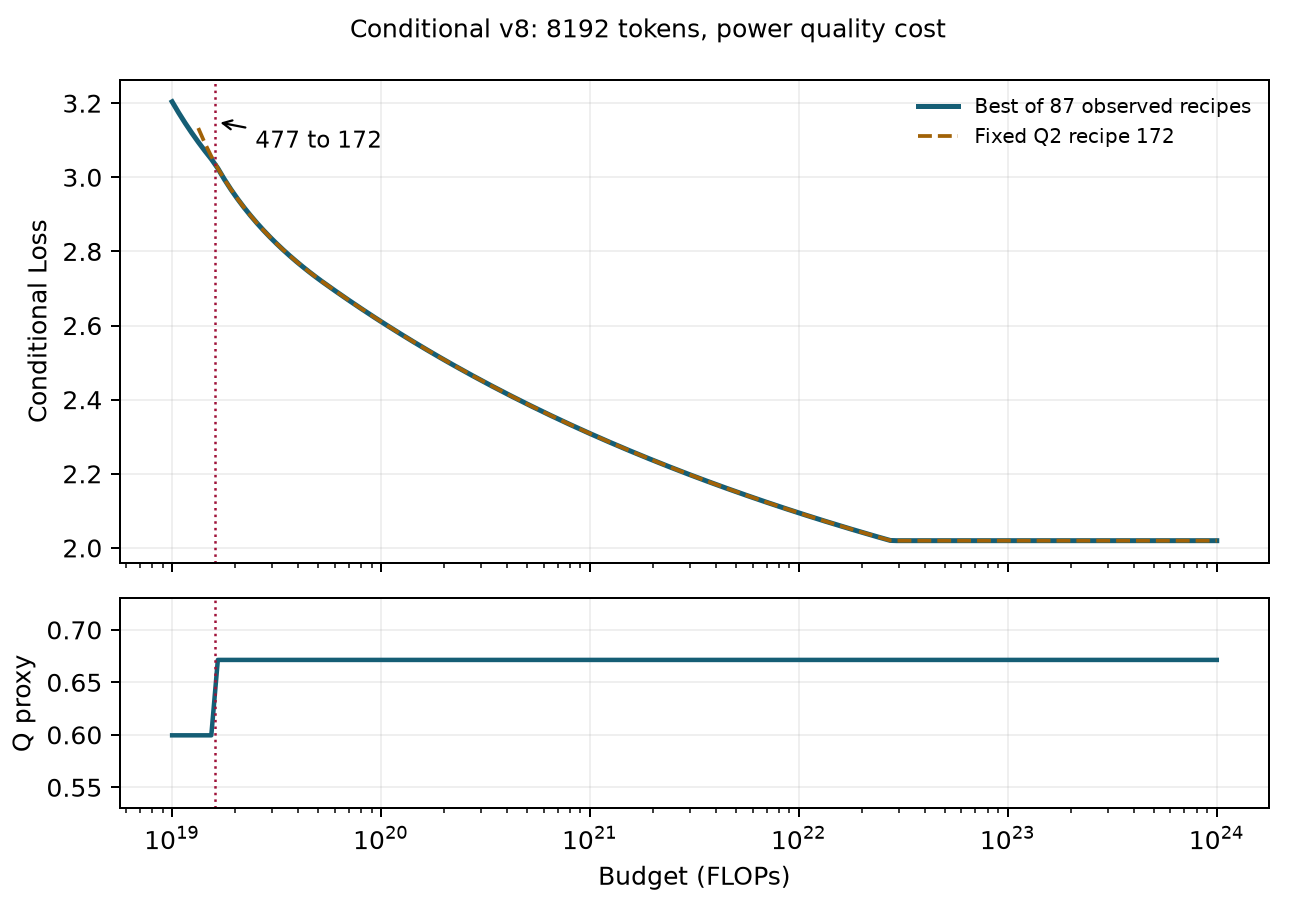
\includegraphics[width=0.86\textwidth]{figures/chm/q3_v8_power_8192.png}
\caption{8192 Token、幂函数质量成本下的条件 Loss 与配比质量代理。
纵虚线是已观测候选中配方 $477\to172$ 的数值切换括区；
曲线只在 v8 共同支持域内绘制。}
\label{fig:q3_v8_budget}
\end{figure}

注意力与基础训练开销的比值由题面公式直接消去 $N,D$：
\begin{equation}
\frac{C_{\rm attention}}{C_{\rm train}}=\frac{L_c}{30000},
\qquad L_{\rm crit}=30000\ {\rm Token}.
\label{eq:q3_v8_context}
\end{equation}
C7 的 2048、8192、131072 Token 分别给出约 0.0683、0.2731、4.3691。
$L_{\rm crit}$ 是两项简化成本相等的位置，不是观测得到的模型能力阈值；
尤其长上下文情景应按稀疏支持谨慎解释。

\subsubsection{数值复核与结论边界}
CYJ v8 的 18 个冻结请求/期望样例在 CHM 本机重放通过；
固定配方的 $10^{22}$ FLOPs、8192 Token、幂成本解与独立 SLSQP
在 Loss 上相差小于 $10^{-8}$。本轮 7 项新检查覆盖精确生产者身份、
跨源标记、支持域、成本分解、预算、有限候选排序和转移括区；
自由 $Q_B$ 模式的最大浮点目标间隙约 $10^{-7}$。
这些误差界只处理\emph{给定模型内的数值求解}，不含 B1/B7 参数、
跨附件映射、配比桥、模型形式或选优造成的总预测误差。
附件 B7 为半合成质量数据；缺少 A/B 成对实验使 Q1 质量和配比响应无法
在同一真实 Loss 坐标中独立识别。因此本文只将表中配置用作
条件规划情景，不给出联合 95\% 区间、真实训练因果收益或 Benchmark 提升断言。
完整表、输入与程序 SHA256、角色和复现命令见
\texttt{outputs/chm/q3\_conditional\_v8/manifest.json}。
